\documentclass{article}

\usepackage{graphicx}
\usepackage{subcaption}
\usepackage{amsmath}
\usepackage{float}
\usepackage{listings}
\usepackage{xcolor}

\lstset{
    language=C,
    basicstyle=\ttfamily\footnotesize,
    keywordstyle=\color{blue},
    stringstyle=\color{red},
    commentstyle=\color{green},
    breaklines=true,
    numbers=left,
    numberstyle=\tiny\color{gray},
    stepnumber=1,
    numbersep=5pt,
    showspaces=false,
    showstringspaces=false,
    tabsize=2
}

\author{Davi de Lima Cruz\\  PROJETO 01-2024.2: Grupo 1}
\title{Relatório: Ampliando e reduzindo imagens por interpolação bilinear}
\date{\today}

\begin{document}
\maketitle

\vfill
\section*{Resumo}
    Este relatório apresenta a implementação de um programa que amplia e reduz imagens por interpolação bilinear. O programa foi implementado em C e utiliza a biblioteca libtiff para ler e escrever imagens no formato TIFF.
     O programa foi testado com imagens de diversos tamanhos e resoluções e os resultados obtidos foram satisfatórios.


\newpage
\section{Discussão Técnica}
\subsection{Formato TIFF}
O formato TIFF é um formato de arquivo de imagem flexível e poderoso que suporta vários tipos de dados,
 incluindo imagens monocromáticas, imagens coloridas e imagens em tons de cinza.
  O formato TIFF é amplamente utilizado em aplicações de imagem e é suportado por muitos programas de edição de imagem.

\subsection{DPI}
DPI (dots per inch) é uma unidade de medida que indica a resolução de uma imagem.
 A resolução de uma imagem é o número de pixels por polegada e é usada para determinar a qualidade da imagem.
  Uma imagem com uma resolução mais alta tem mais detalhes e é mais nítida do que uma imagem com uma resolução mais baixa.
   A resolução de uma imagem é importante ao imprimir a imagem, pois determina a qualidade da impressão.
   Podemos descobrir a resolução da nova imagem a partir da resolução da imagem original e do fator de escala, que é opbido pela razão dos DPIs da imagem original e da imagem modificada.
   \begin{equation}
    fator\_escala  = \frac{DPI_{original}}{DPI_{nova}}
   \end{equation}
\subsection{Interpolação Bilinear}
A interpolação bilinear é um método de interpolação que calcula o valor de um pixel interpolado com base nos valores dos pixels vizinhos.
 O método é usado para aumentar ou reduzir o tamanho de uma imagem e é amplamente utilizado em aplicações de processamento de imagem.
A interpolação bilinear é um método simples e eficaz para aumentar ou reduzir o tamanho de uma imagem e produz resultados de alta qualidade.
    Dado as posições $x_1$, $x_2$, $y_1$ e $y_2$ dos pixels vizinhos, o valor do pixel interpolado é calculado pela fórmula:

        \begin{eqnarray}
            I(x, y) = \frac{1}{(x_2-x_1)(y_2-y_1)}( f(x_1, y_1)(x_2-x)(y_2-y) + \\
             + f(x_2, y_1)(x-x_1)(y_2-y) + \nonumber \\
             + f(x_1, y_2)(x_2-x)(y-y_1)+  \nonumber\\ 
             + f(x_2, y_2)(x-x_1)(y-y_1) ) \nonumber
        \end{eqnarray}

\section{Discussão dos Resultados}
\begin{figure}[h]
    \centering
        \begin{subfigure}[b]{0.3\textwidth}
            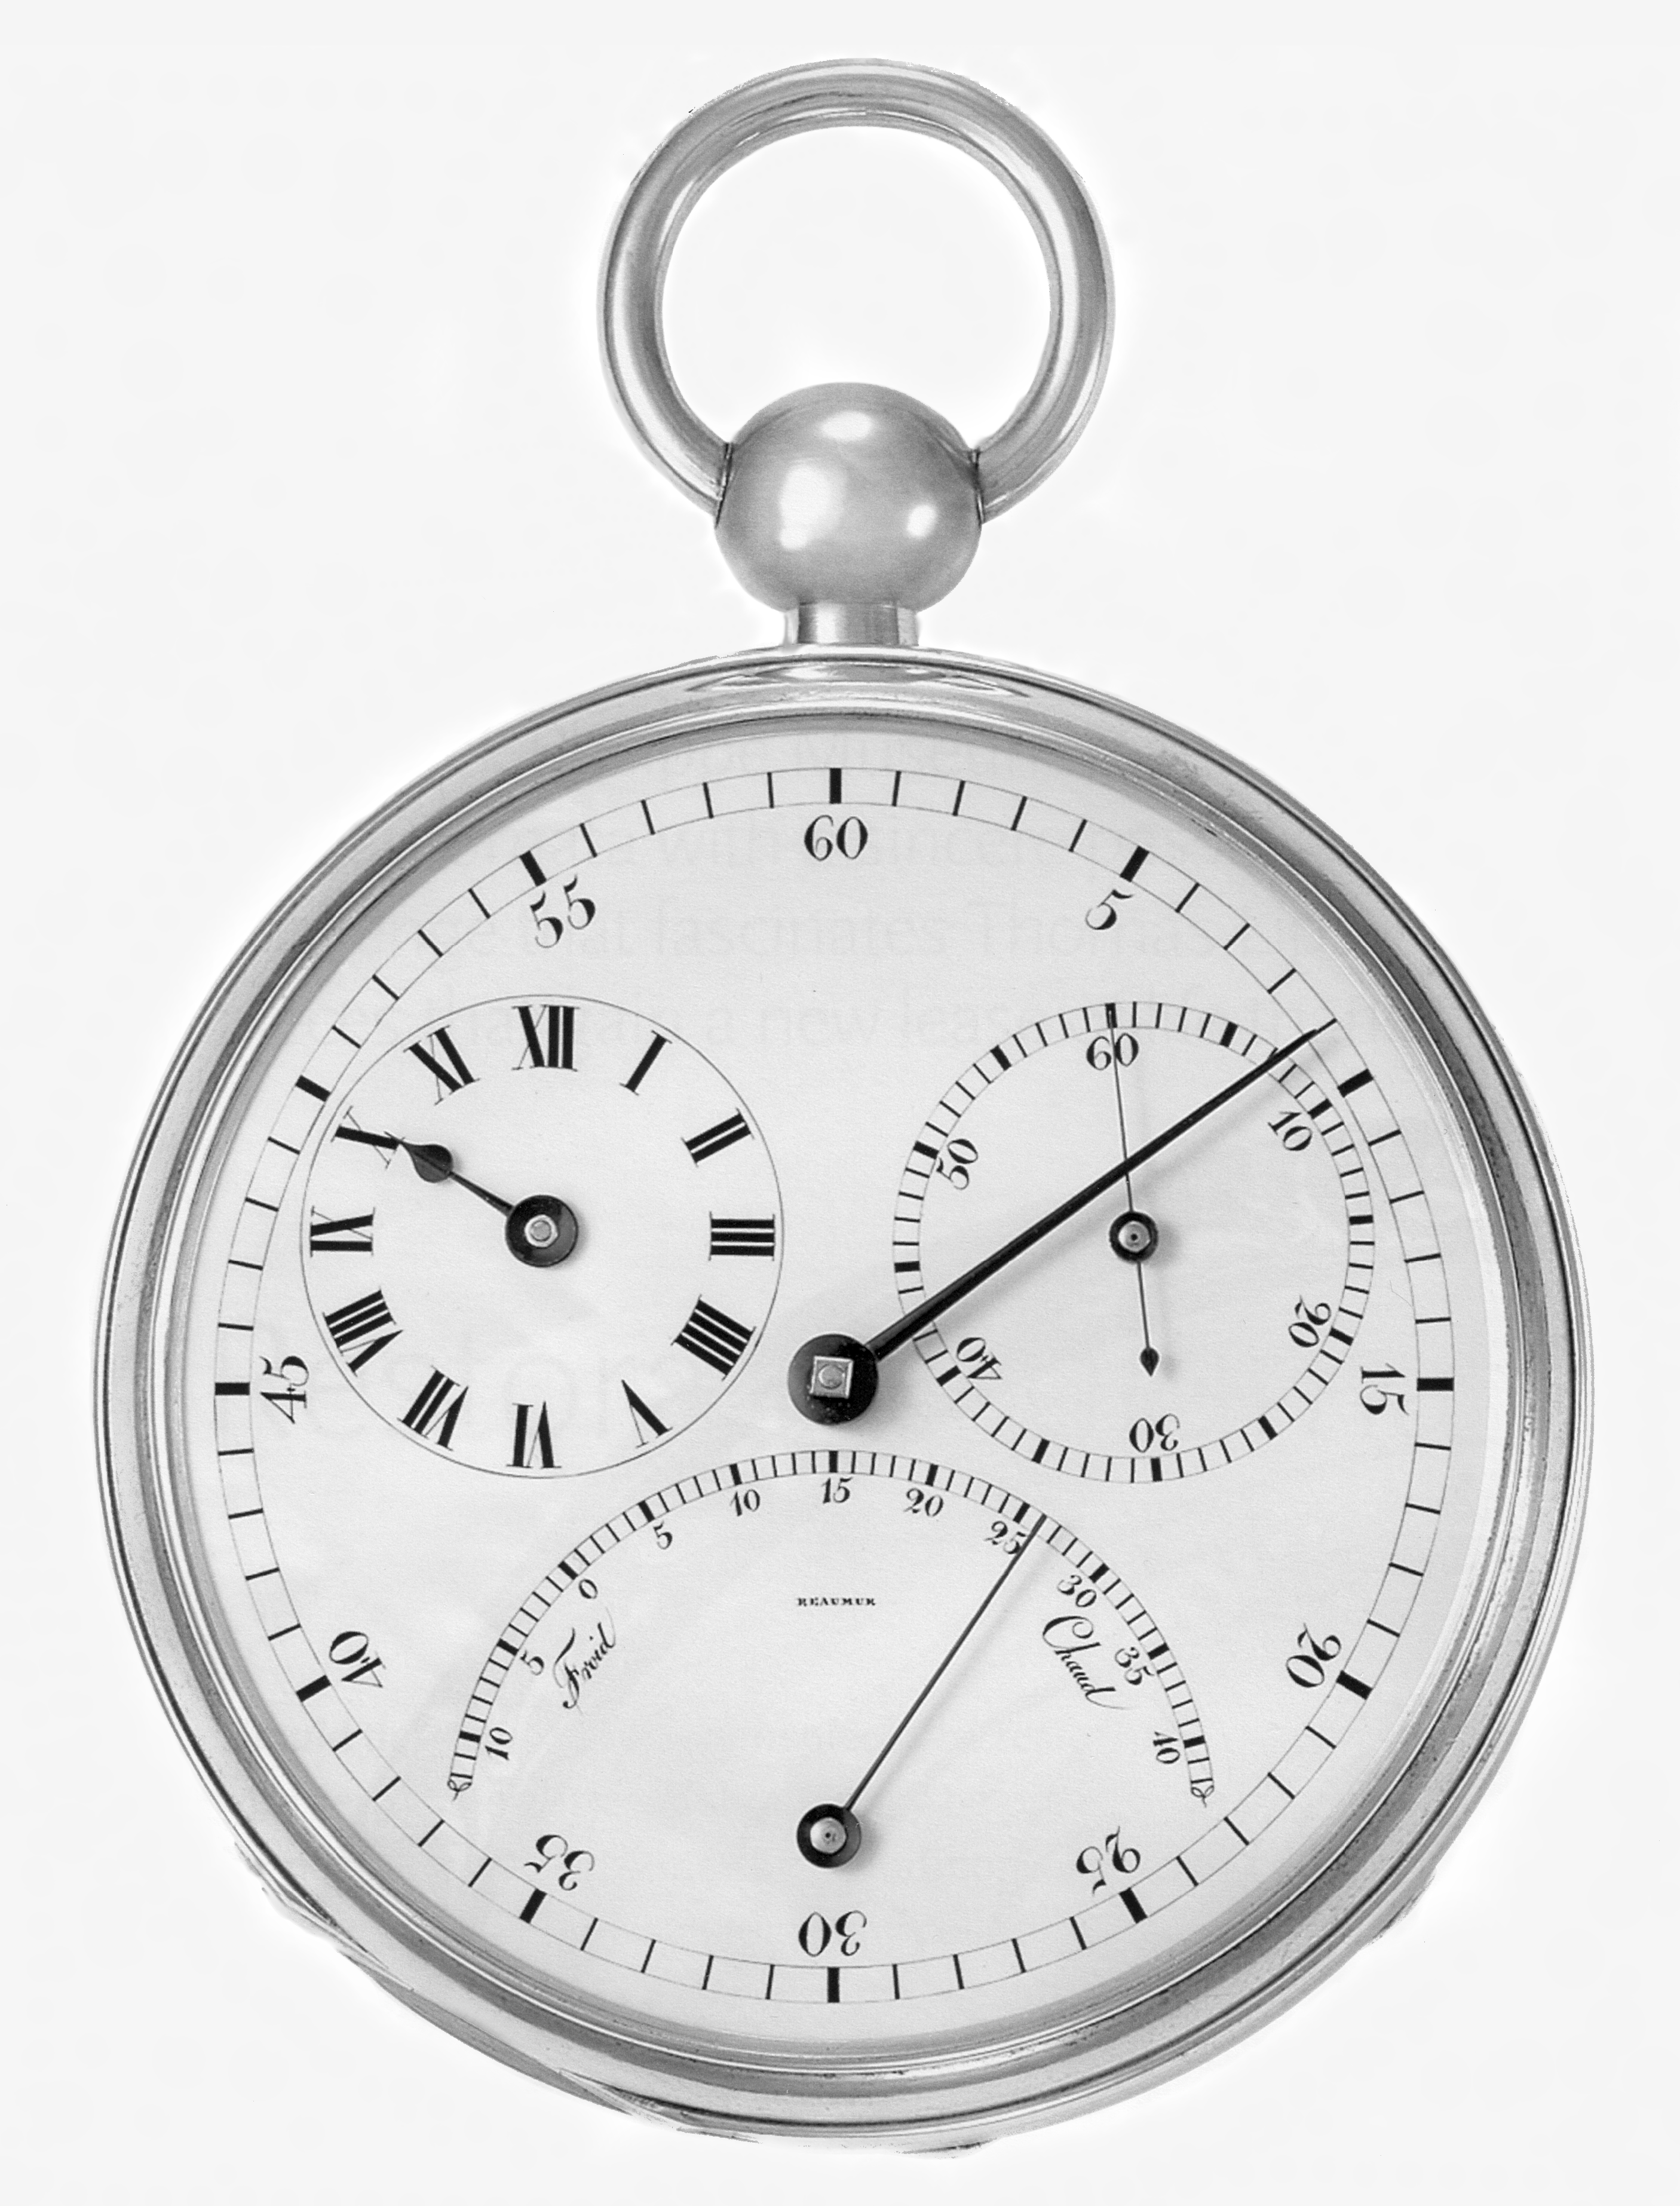
\includegraphics[width=\textwidth]{figures/clock_original.tif.png}
            \caption{Imagem original.}
            \label{fig:clock_original}
        \end{subfigure}
        \hfill
        \begin{subfigure}[b]{0.3\textwidth}
            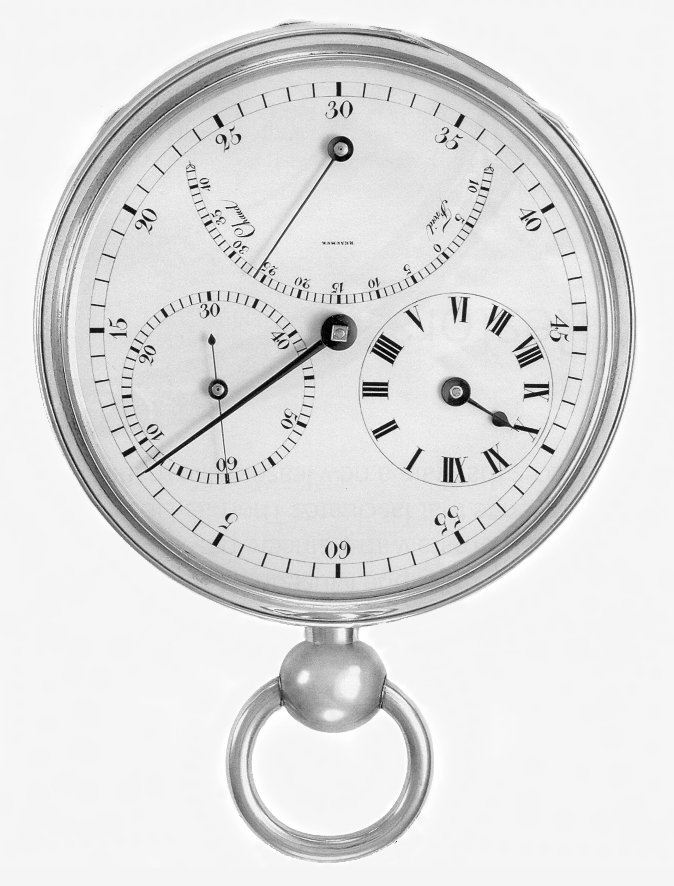
\includegraphics[width=\textwidth, angle=180]{figures/clock_a.tif.png}
            \caption{Imagem com 300 dpi.}
            \label{fig:clock_300dpi}
        \end{subfigure}
        \hfill
        \begin{subfigure}[b]{0.3\textwidth}
            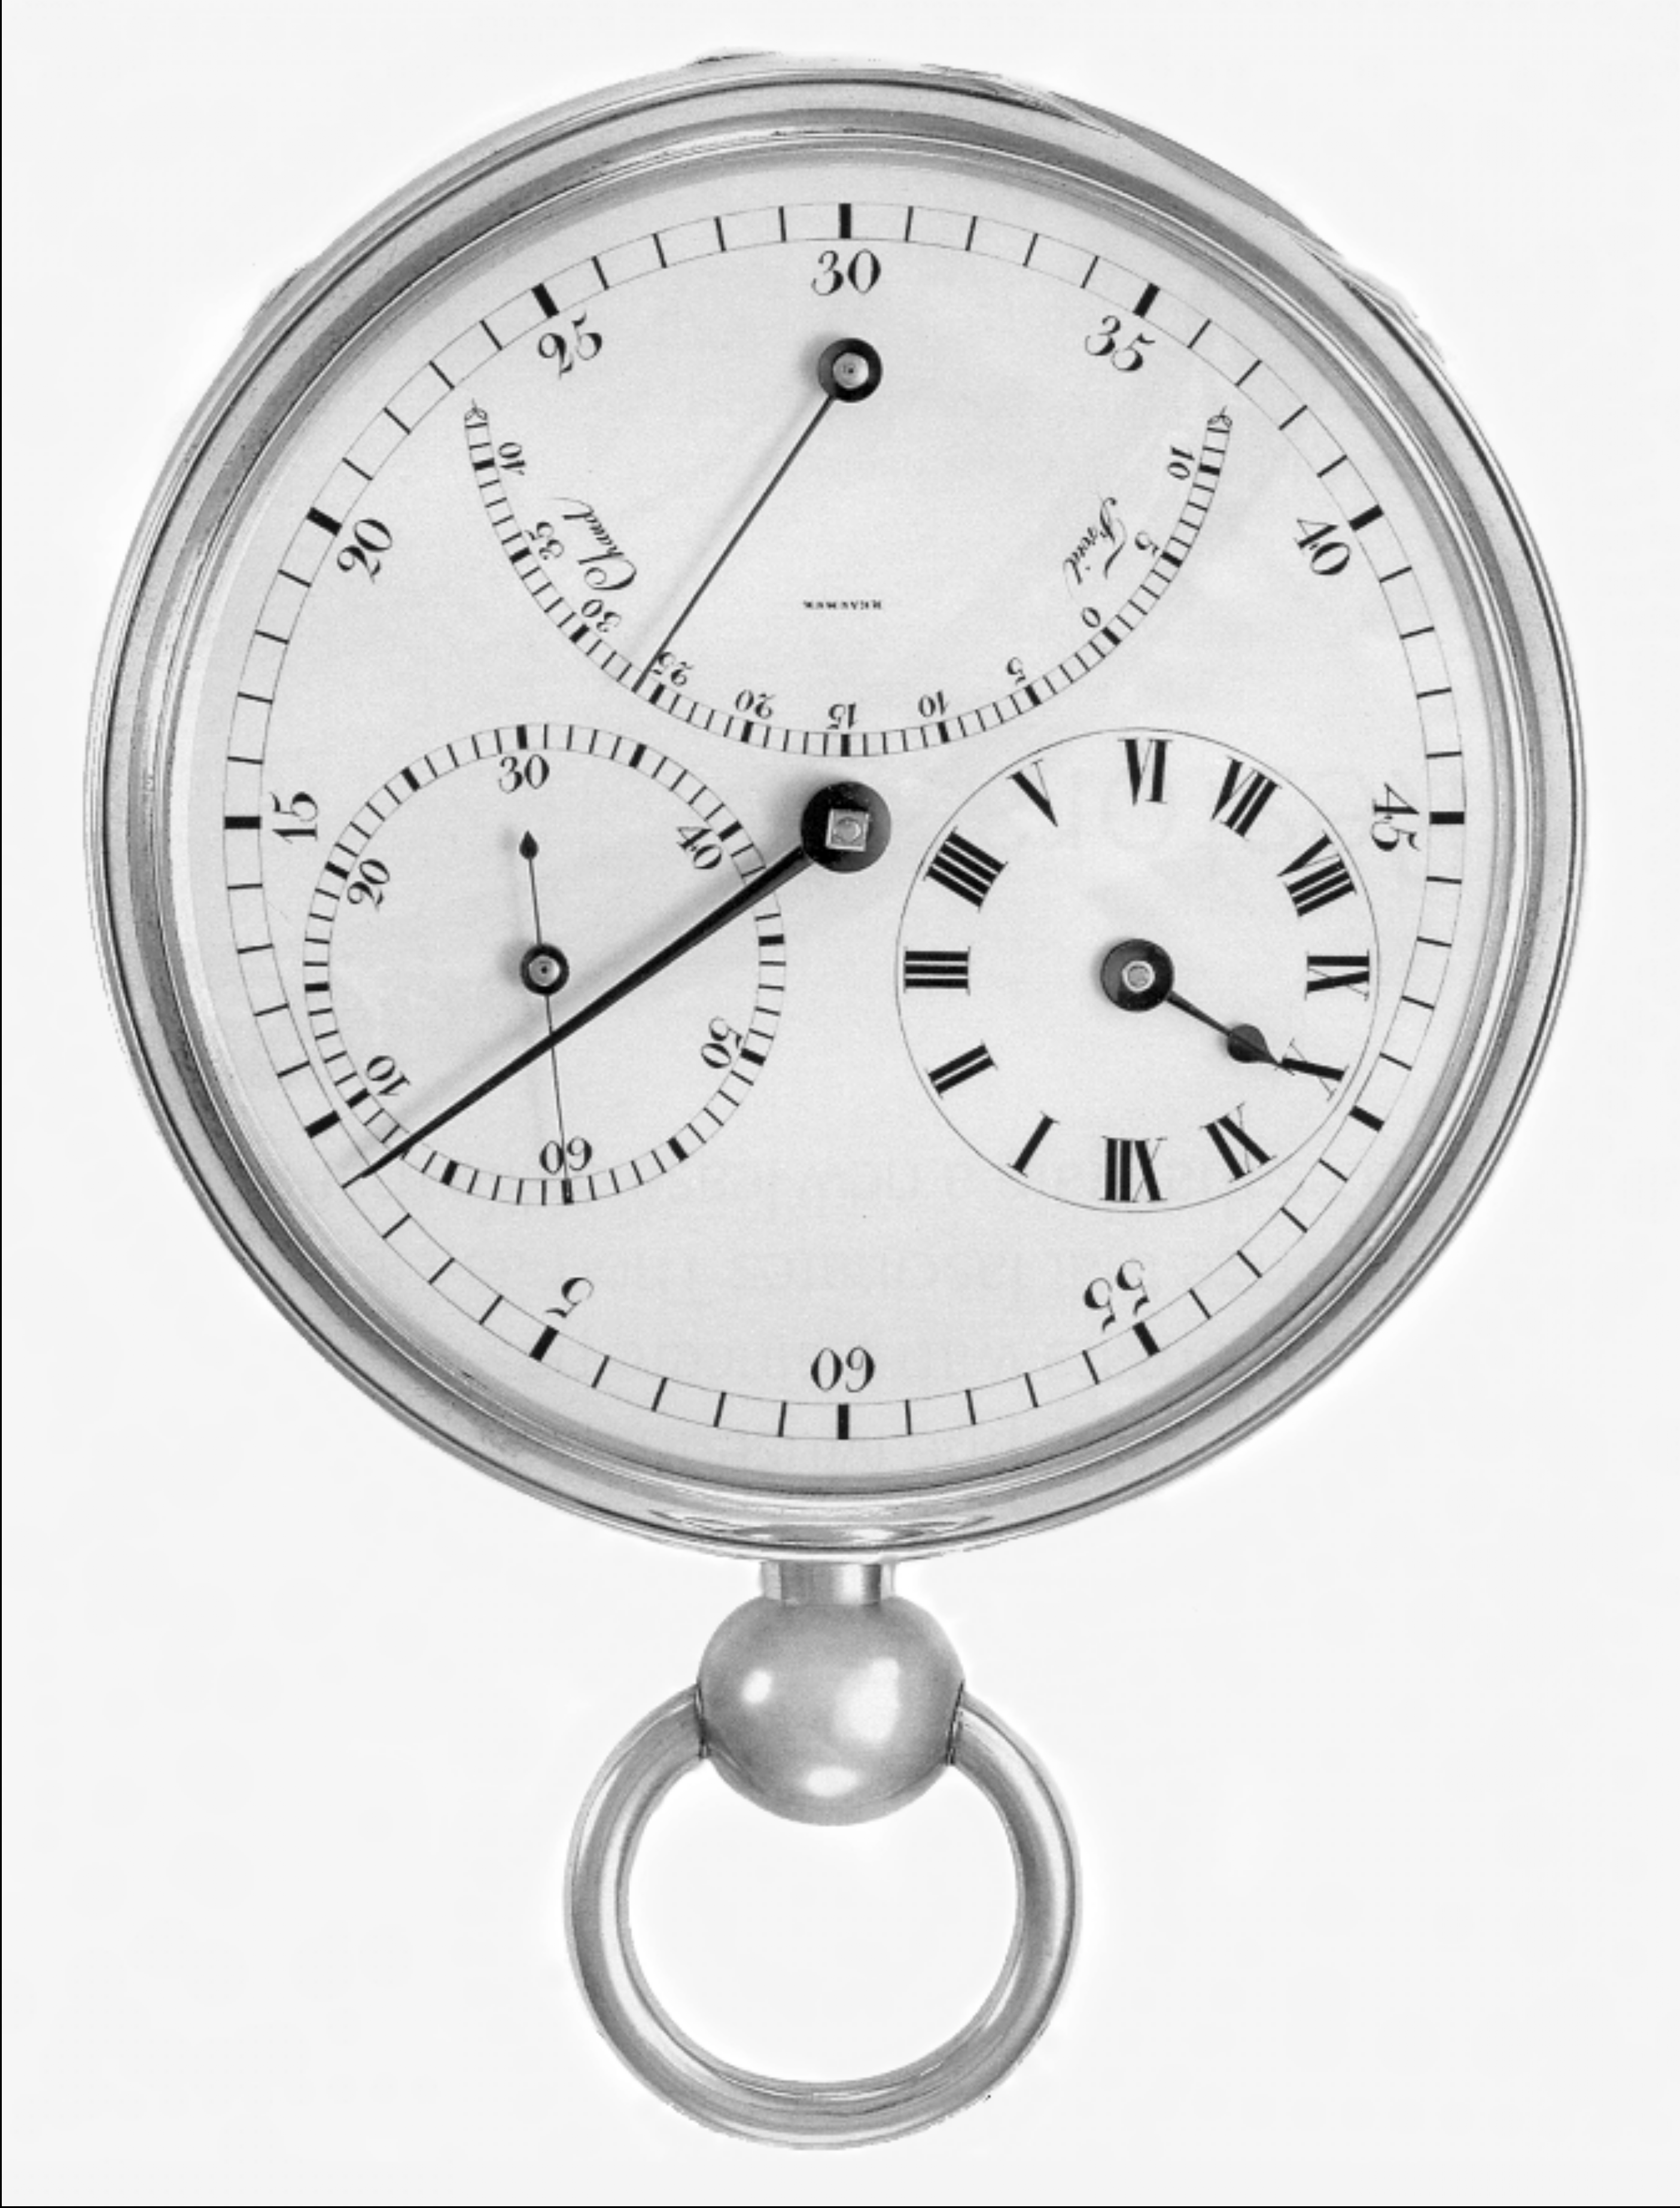
\includegraphics[width=\textwidth, angle=180]{figures/clock_b.tif.png}
            \caption{Imagem com 1250 dpi.}
            \label{fig:clock_1250dpi}
        \end{subfigure}
        \caption{Comparação entre as imagens do relógio.}
        \label{fig:clock_comparison}
\end{figure}
Para o relógio, as diferenças são pouco perceptíveis, mas a imagem com 1250 dpi (Figura \ref{fig:clock_1250dpi}) é um pouco menos nítida que a imagem original (Figura \ref{fig:clock_original}). Isso ocorre porque a primeira interpolação perdeu informações da imagem original.
A seguir, apresentamos um zoom do centro do relógio nas duas imagens com 1250 dpi:
\begin{figure}[H]
    \centering
        \begin{subfigure}[b]{0.45\textwidth}
            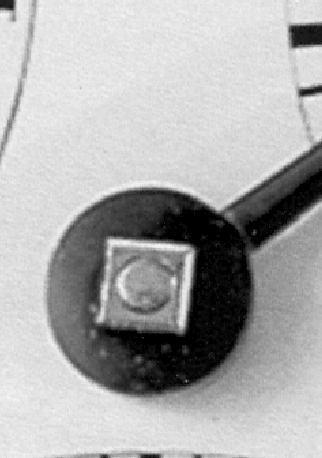
\includegraphics[width=0.6\textwidth]{figures/clock_original_zoom.tif.png}
            \caption{Imagem original.}
            \label{fig:clock_original_zoom}
        \end{subfigure}
        \begin{subfigure}[b]{0.45\textwidth}
            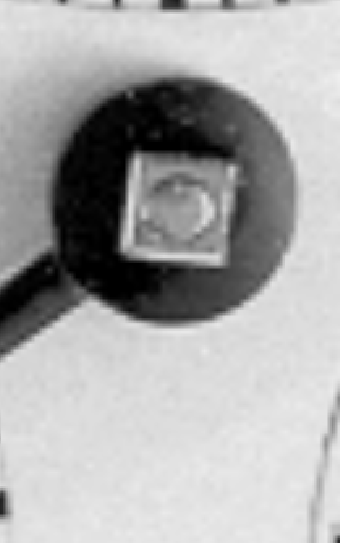
\includegraphics[width=0.6\textwidth, angle=180]{figures/clock_b_zoom.tif.png}
            \caption{Imagem com 1250 dpi.}
            \label{fig:clock_1250dpi_zoom}
        \end{subfigure}
        \caption{Comparação entre as imagens do relógio com zoom.}
        \label{fig:clock_zoom_comparison}
\end{figure}
Podemos ver que o relógio original (Figura \ref{fig:clock_original_zoom}) tem muito mais detalhes do que a imagem transformada com 1250 dpi (Figura \ref{fig:clock_1250dpi_zoom}).
\begin{figure}[H]
    \centering
        \begin{subfigure}[b]{0.3\textwidth}
            \includegraphics[width=\textwidth]{figures/moon_original.tif.png}
            \caption{Imagem original.}
            \label{fig:moon_original}
        \end{subfigure}
        \hfill
        \begin{subfigure}[b]{0.3\textwidth}
            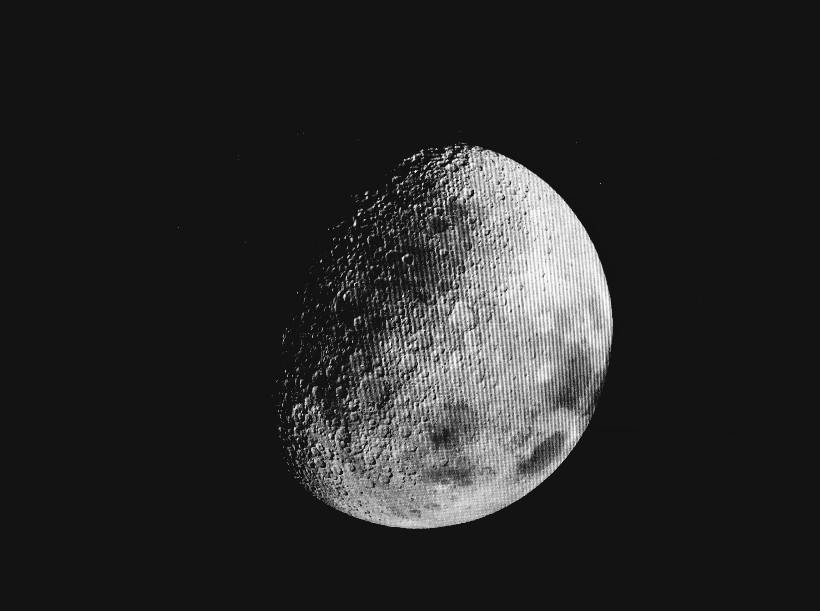
\includegraphics[width=\textwidth, angle=180]{figures/moon_a.tif.png}
            \caption{Imagem com 10 dpi.}
            \label{fig:moon_10dpi}
        \end{subfigure}
        \hfill
        \begin{subfigure}[b]{0.3\textwidth}
            \includegraphics[width=\textwidth, angle=180]{figures/moon_b.tif.png}
            \caption{Imagem com 100 dpi.}
            \label{fig:moon_100dpi}
        \end{subfigure}
        \caption{Comparação entre as imagens da lua.}
        \label{fig:moon_comparison}
\end{figure}
A imagem da lua com 10 dpi (Figura \ref{fig:moon_10dpi}) é muito pixelada, enquanto a imagem com 100 dpi (Figura \ref{fig:moon_100dpi}) é mais nítida, mas ainda apresenta pixelização. Isso ocorre porque a imagem original (Figura \ref{fig:moon_original}) é muito pequena e a interpolação não consegue recuperar as informações perdidas.

\begin{figure}[H]
    \centering
        \begin{subfigure}[b]{0.3\textwidth}
            \includegraphics[width=\textwidth]{figures/city_original.tif.png}
            \caption{Imagem original.}
            \label{fig:city_original}
        \end{subfigure}
        \hfill
        \begin{subfigure}[b]{0.3\textwidth}
            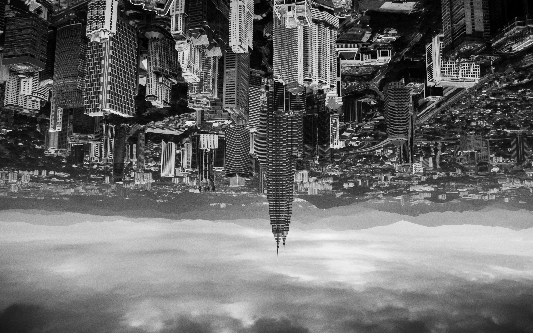
\includegraphics[width=\textwidth, angle=180]{figures/city_a.tif.png}
            \caption{Imagem com 10 dpi.}
            \label{fig:city_10dpi}
        \end{subfigure}
        \hfill
        \begin{subfigure}[b]{0.3\textwidth}
            \includegraphics[width=\textwidth, angle=180]{figures/city_b.tif.png}
            \caption{Imagem com 100 dpi.}
            \label{fig:city_100dpi}
        \end{subfigure}
        \caption{Comparação entre as imagens da cidade.}
        \label{fig:city_comparison}
\end{figure}
A cidade apresentou o pior resultado. A imagem com 10 dpi (Figura \ref{fig:city_10dpi}) é extremamente pixelada, e a imagem com 100 dpi (Figura \ref{fig:city_100dpi}) também é pixelada e apresenta detalhes distorcidos.
 Resumindo os resultados, a interpolação bilinear é eficaz para aumentar e diminuir o tamanho de uma imagem se não tiver muitos detalhes. A qualidade da imagem ampliada depende da resolução da imagem original e do fator de escala. Se a imagem original for muito pequena, a interpolação não conseguirá recuperar as informações perdidas e a imagem ampliada será pixelada. Se a imagem original for grande, a interpolação produzirá uma imagem ampliada de alguma qualidade.
\section{Código Fonte em C}
\lstinputlisting[language=C, caption={Código fonte do programa em C.}]{src/main.c}
\end{document}